\begin{figure}%{l}{0pt}%[0.4\textwidth]
%\begin{center}
  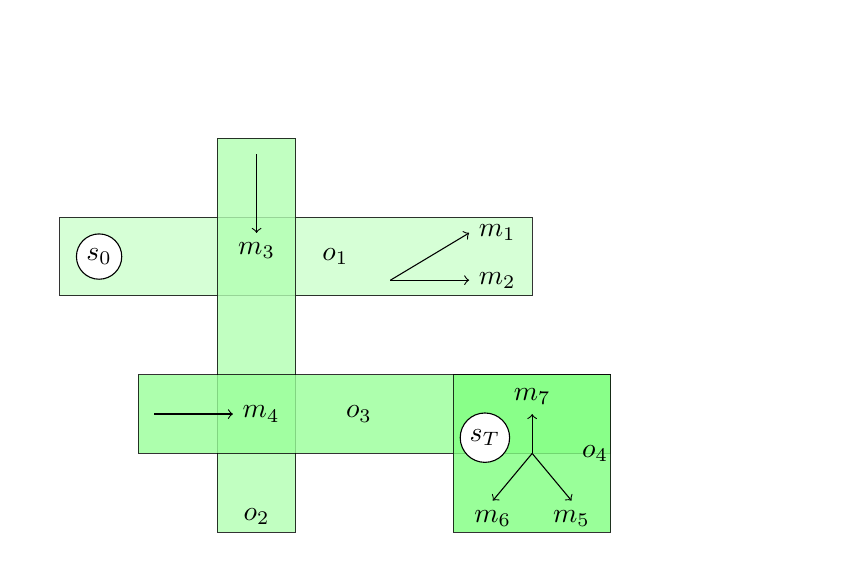
\begin{tikzpicture}
  \tikzstyle{every state}=[fill=gray!20!white,shape=rounded rectangle]
  
    \draw [fill=green!20, opacity=0.8] (0,0) rectangle (6,1);
    \node at (3.5, 0.5) {$o_1$};
    \node[fill=white!80, circle,inner sep=0.2em, draw] at (0.5, 0.5) {${\color{black}s_0}$};
    \draw[->] (4.2, 0.2) -- (5.2, 0.8) node[right] {$m_1$};
    \draw[->] (4.2, 0.2) -- (5.2, 0.2) node[right] {$m_2$};
    
    \draw [fill=green!30, opacity=0.8] (2,2) rectangle (3,-3);
    \node at (2.5, -2.8) {$o_2$};
    \draw[->] (2.5, 1.8) -- (2.5, 0.8) node[below] {$m_3$};
    
    \draw [fill=green!40, opacity=0.8] (1, -1) rectangle (7, -2);
    \node at (3.8, -1.5) {$o_3$};
    \draw[->] (1.2, -1.5) -- (2.2, -1.5) node[right] {$m_4$};
    
    \draw [fill=green!50, opacity=0.8] (5, -1) rectangle (7, -3);
    \node at (6.8, -2) {$o_4$};
    \draw[->] (6, -2) -- (6.5, -2.6) node[below] {$m_5$};
    \draw[->] (6, -2) -- (5.5, -2.6) node[below] {$m_6$};
    \draw[->] (6, -2) -- (6, -1.5) node[above] {$m_7$};
    \node[fill=white,circle,inner sep=0.2em, draw] at (5.4, -1.8)
    {${\color{black}s_T}$};
    
	\draw [dashed, draw=white] (6.6, 1.4) rectangle (7.4, -0.4);
    \draw [dashed, draw=white] (2.1, 3.4) rectangle (2.9, 2.6);
    \draw [dashed, draw=white] (-0.4, -1.1) rectangle (0.4, -1.9);
	\draw [dashed, draw=white] (7.6, -2.9) rectangle (9.9, -1.1);
      
  \end{tikzpicture}                        
%\end{center}
  \caption{Robotic motion planning problem modelled as a reachability question}
  \label{fig:robocop}
\end{figure}
